\section{Описание}

{\large\bfseries Принцип работы программы:} \\
Необходимо разработать программу, которая для сжатия заданного файла последовательно применяет следующие алгоОснритмы сжатия:
\begin{enumerate}
    \item {\bfseries  Burrows-Wheeler transform}
        
    \item {\bfseries Move-To-Front}
    
    \item {\bfseries Run-Length Encoding}
    
    \item {\bfseries Код Хаффмана}
    
\end{enumerate} \\

Такая последоательность обусловленная тем, что {\it преобразоавние Барроуза-Уилера} преобразует данные к виду, в котором часто встречаются последовательности поторяющихся символов. С такими последоательностями хорошо работают алгоритмы {\it MTF} и {\it RLE} для последующего преобразования {алгоритмом Хаффмана}, который после оптимизирует кодирование повторяющихся последовательностей, полученных после {\it BWT}  что улучшает степень сжатия. \cite{mtf} \\

{\large\bfseries Принцип работы программы:} \\
Основной принцип работы заключается в следующей последовательности шагов:
\begin{enumerate}
    \item Открытие файлового потока, который необходимо сжать
    \item Создание временного файла для размещения в нем инормации из потока
    \item Последовательное применение алгоритмов сжатия к временному файлу. После применения каждого алгоритма преобразоавния на выходе получается новый временный файл с результатом работы алгоритма, после чего закрывается и удаляется старый временный файл.
    \item После применения всех алгритмов преобразоавния на основе полученного результпата сжатия ормируется результирующий файл, который будет содерать необходимую информацию и результат сжатия.
\end{enumerate} \\

{\large\bfseries Преобразование Барроуза-Уилера:} \\
\enquote{Преобразование Барроуза — Уилера (англ. Burrows-Wheeler transform) — алгоритм, используемый для предварительной обработки данных перед сжатием, разработанный для улучшения эффективности последующего кодирования. Преобразование Барроуза — Уилера меняет порядок символов во входной строке таким образом, что повторяющиеся подстроки образуют на выходе идущие подряд последовательности одинаковых символов.} \cite{bwt} \\

Преобразование выполняется в три этапа:
\begin{enumerate}
    \item Составляется таблица всех циклических сдвигов входной строки.
    \item Производится лексикографическая (в алфавитном порядке) сортировка строк таблицы.
    \item В качестве выходной строки выбирается последний столбец таблицы преобразования и номер строки, совпадающей с исходной.
\end{enumerate} \\

Наивная реализация первых двух этапов описанного алгоритма будет иметь как пространстенную, так и временную сложность $O(n^2)$. Что непозволительно долго.\\
Поэтому я воспользовался идеей применения суффиксного массива, который по определению явяется перестанокой всех суффиксов строки в лексикографическом порядке. Сущестуют довольно сложные алгоритмы, например описанный в \cite{suf} {\it алгоритм Карккайнена-Сандерса}, произодящие построение суффиксного массива за время $O(n)$, однако при этом встает нетривиальная задача преобразования суффиксного массива к перестаноке циклических сдвигов. \\
Поэтому я решил пожертвоать асимптотикой и остановился на описанном в \cite{emax} алгоритме построения суффиксного массива за $O(n\log{n})$, который обладает полезным свойством: он строит массив на основе сортировки циклических сдвигов путем добавления к алгоритму терминального символа, что делает этот метод идеально адаптируемым к нашей задаче, так как мы получим необходимый результат лишь пропустив шаг добавления терминала. \\
К приятным свойствам алгоритма можно отнести и то, что он требует $O(n)$ памяти. \\ 

Опишем алгоритм построения массива. Как сказано в \cite{emax}: \\
\enquote{На нулевой фазе мы должны отсортировать циклические подстроки длины 1, т.е. отдельные символы строки, и разделить их на классы эквивалентности (просто одинаковые символы должны быть отнесены к одному классу эквивалентности). Это можно сделать тривиально, например, сортировкой подсчётом. Для каждого символа посчитаем, сколько раз он встретился. Потом по этой информации восстановим отсортированный массив. После этого, проходом по массиву и сравнением символов, строится массив классов эквивалентности. \\
Далее, пусть мы выполнили $k-1$-ю фазу, теперь научимся за $O(n)$ выполнять следующую, $k$-ю, фазу. Поскольку фаз всего $O(\log{n})$, это даст нам требуемый алгоритм с временем $O(n\log{n})$.
Для этого заметим, что циклическая подстрока длины $2^k$ состоит из двух подстрок длины $2^{k-1}$, которые мы можем сравнивать между собой за $O(1)$, используя информацию с предыдущей фазы — номера классов эквивалентности. Таким образом, для подстроки длины $2^k$, начинающейся в позиции $i$, вся необходимая информация содержится в паре чисел классов эквивалентности для позиции $i$ и $i + 2^{k-1}$.\\
Это даёт нам весьма простое решение: отсортировать подстроки длины $2^k$ просто по этим парам чисел, это и даст нам требуемый порядок. \\
Воспользуемся здесь приёмом, на котором основана так называемая цифровая сортировка: чтобы отсортировать пары, отсортируем их сначала по вторым элементам, а затем — по первым элементам (но уже обязательно стабильной сортировкой, т.е. не нарушающей относительного порядка элементов при равенстве).} \\

После построения массива сдигов выполнить 3-ий шаг преобразоания $BWT$ - трииальная задача.\\

При декодировании воспользуемся оптимизацией наивного алгоритма. Наиный алгоритм из \cite{bwt}: \enquote{Выпишем в столбик нашу преобразованную последовательность символов. Запишем её как последний столбик предыдущей матрицы (при прямом преобразовании Барроуза — Уилера), при этом все предыдущие столбцы оставляем пустыми. Далее построчно отсортируем матрицу, затем в предыдущий столбец запишем преобразоанную последовательность. Опять построчно отсортируем матрицу. Продолжая таким образом, можно восстановить полный список всех циклических сдвигов строки, которую нам надо найти. Выстроив полный отсортированный список сдвигов, выберем строку с номером, который нам был изначально дан. В итоге мы получим искомую строку.} \\ 

Оптимизация наивного алгоритма из \cite{bwt}: \enquote{Заметим, что при каждом проявлении неизвестного столбца выполнялись одни и те же действия. К предыдущему приписывался новый столбец и имеющиеся данные сортировались. На каждом шаге к строке, которая находилась на i-ом месте, приписывался в начало i -ый элемент столбца входных данных. Пусть изначально известно, каким по порядку является приписанный в начало символ (то есть каким по порядку в столбце). Из предыдущего шага известно, какое место занимала строка без этого первого символа (i -ое). Тогда несложно заметить, что при выполнении такой операции строка с номером i всегда будет перемещаться на позицию с номером j. \\
Поскольку в нашем алгоритме новый столбец приписывается в начало, то мы из состояния i (левый столбец) переходим в состояние j (правый). Для того, чтобы восстановить строку, нам необходимо от последней такой цифры по пути из j в i восстановить строку. } \\

Описанный в \cite{bwt} алгоритм декодирования дает сложность $O(n+m)$, где $m$ - размер алфавита. \\


{\large\bfseries Преобразоавание MTF:} \\
\enquote{Преобразование MTF (англ. move-to-front, движение к началу) — алгоритм кодирования, используемый для предварительной обработки данных (обычно потока байтов) перед сжатием, разработанный для улучшения эффективности последующего кодирования.}\cite{mtf} \\

Мы будем использовать наивный способ реализации алгоритма, описанного в \cite{mtf}: \enquote{Изначально каждое возможное значение байта записывается в список (алфавит), в ячейку с номером, равным значению байта, т.е. $(0,1,2,3,...,255)$. В процессе обработки данных этот список изменяется. По мере поступления очередного символа на выход подается номер элемента, содержащего его значение. После чего этот символ перемещается в начало списка, смещая остальные элементы вправо.}  \\

Изменяющийся алфавит реализуем при помощи структуры - список. \\

Декодирование будет производится последовательно аналогично шагам кодирования.\\

{\large\bfseries Кодирование длинн серий:} \\
\enquote{Кодирование длин серий (англ. run-length encoding, RLE) или кодирование повторов — алгоритм сжатия данных, заменяющий повторяющиеся символы (серии) на один символ и число его повторов. Серией называется последовательность, состоящая из нескольких одинаковых символов. При кодировании (упаковке, сжатии) строка одинаковых символов, составляющих серию, заменяется строкой, содержащей сам повторяющийся символ и количество его повторов.}\cite{wiki} \\ 

При реализации будем последовательно считать либо количество подряд идущих неповторяющихся символов, либо неповторяющихся символов, записываем полученное число перед каждой серией: отрицательное если серия неповторяющихся символов и положительное если серия повторяющихся, после чего помещаем серию после отрицательного числа или один повторяющийся после положительного. \\

Интересным моментом является то, что мы кодируем подсчитываемое число одним байтом, что дает нам закодировать серии до 127 повторяющихся символов и до 128 неповторяющихся, после чего будет необходимо обнулить счетчик и рассматривать дальнейшую последовательность символов как новую серию.\\

Декодирование происходит нивным методом: считываем размер серии, и если он полоительный выписываем нужное количество раз повторяющийся символ, иначе выписывем указанное количество симолов после числа из входной последовательности. \\

{\large\bfseries Алгоритм Хаффмана:} \\
\enquote{Идея, положенная в основу кодировании Хаффмана, основана на частоте появления символа в последовательности. Символ, который встречается в последовательности чаще всего, получает новый очень маленький код, а символ, который встречается реже всего, получает, наоборот, очень длинный код.}\cite{habr} \\

Важное свойсво кодирования: каждый код символа не является префиксом для кода другого символа. \\

Алгоритм будет использовать очередь с приоритетом для построения дерева. Приоритетом будет выступать частота встречи символа в последовательности.\\
Описание алгоритма на основе материала из \cite{habr}:
\begin{enumerate}
    \item Для начала посчитаем частоты всех символов
    \item После вычисления частот мы создадим узлы бинарного дерева для каждого знака и добавим их в очередь, используя частоту в качестве приоритета.
    \item Теперь мы достаём два первых элемента из очереди и связываем их, создавая новый узел дерева, в котором они оба будут потомками, а приоритет нового узла будет равен сумме их приоритетов. После этого мы добавим получившийся новый узел обратно в очередь.
    \item После того, как мы свяжем два последних элемента, получится итоговое дерево
    \item Теперь, чтобы получить код для каждого символа, надо просто пройтись по дереву, и для каждого перехода добавлять 0, если мы идём влево, и 1 — если направо
\end{enumerate}

После построения дерева построим таблицу кодов при помощи обхода дерева для быстрого кодирования символа. \\

Дерево мы сохраним в файле для возмоности декодирования последовательности. \\

При декодировании необходимо считать дерево из входной последоавтельности, после чего в заисимости от встреченного бита во входной последовательности будем двигаться влево или вправо пока не придем в лист. Если попадаем в лист выписываем полученный символ в выходную последовательность и возвращаемся в корень. \\

\pagebreak

\section{Демонстрация работы:}

Продемонстрируем работу алгоритма на примере текстового файла, содержащего в себе строку \enquote{abrakadabra}.

Исходный буфер после считывания из файла будет выглядеть следующим образом:

{\center{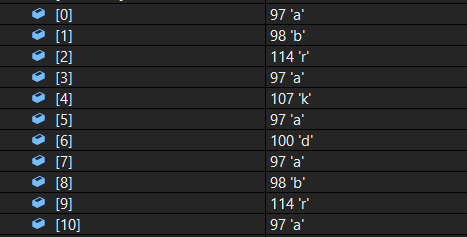
\includegraphics[scale = 0.55]{src/Screenshot_1.png}}} \\

После работы алгоритма BWT исходная строка будет преобразована в следующую последовательность, содержащую в себе преобразованную строку и позицию исходной строки в таблице отсортированных циклических сдвигов:

{\center{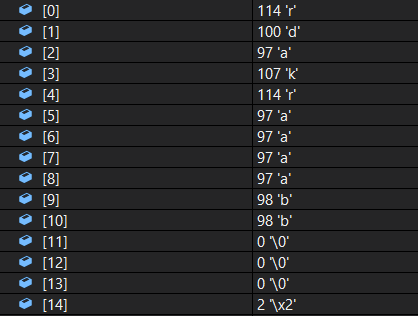
\includegraphics[scale = 0.55]{src/Screenshot_2.png}}}\\

После работы в начало добавляется размер закодированного буффера и добавлен в выходной временный файл вместе с преобразованной таблицей.\\

Считываем буффер из временного файла:

{\center{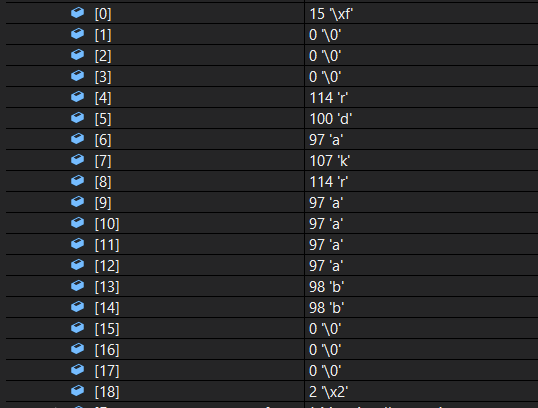
\includegraphics[scale = 0.55]{src/Screenshot_3.png}}} \\

После преобразования алгоритмом MTF отметим, что размер выходной последовательности не поменялся:

{\center{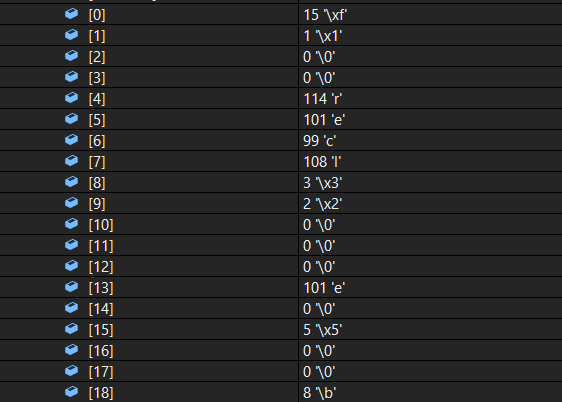
\includegraphics[scale = 0.55]{src/Screenshot_4.png}}}\\

Снова считаем буффер из временного файла:

{\center{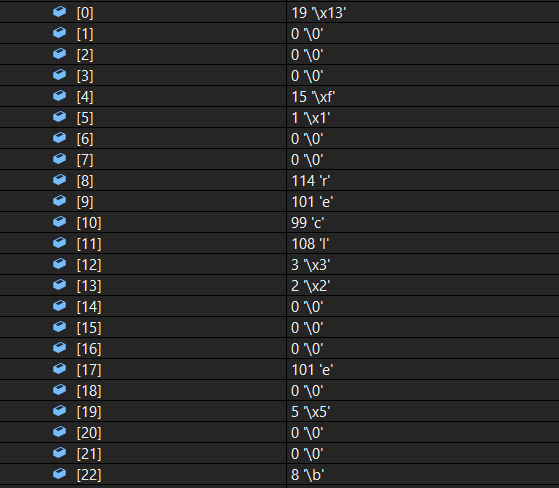
\includegraphics[scale = 0.55]{src/Screenshot_5.png}}}\\

\pagebreak

После работы RLE у нас вся последовательность преобразовалась в вид, в котором идут сначала либо положительные, либо отрицательные числа, после которых идут либо один символ, если число положительное, либо количество неповторяющихся символов равное взятому абсолютному значению числа:

{\center{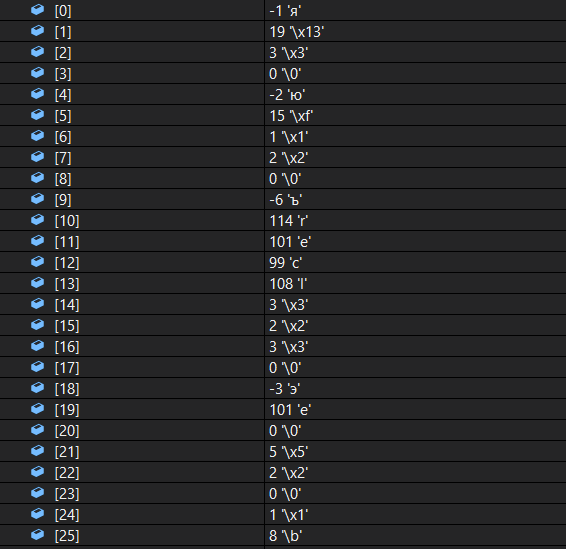
\includegraphics[scale = 0.5]{src/Screenshot_6.png}}}\\

Считываем буффер из временного файла для последнего преобразования:

{\center{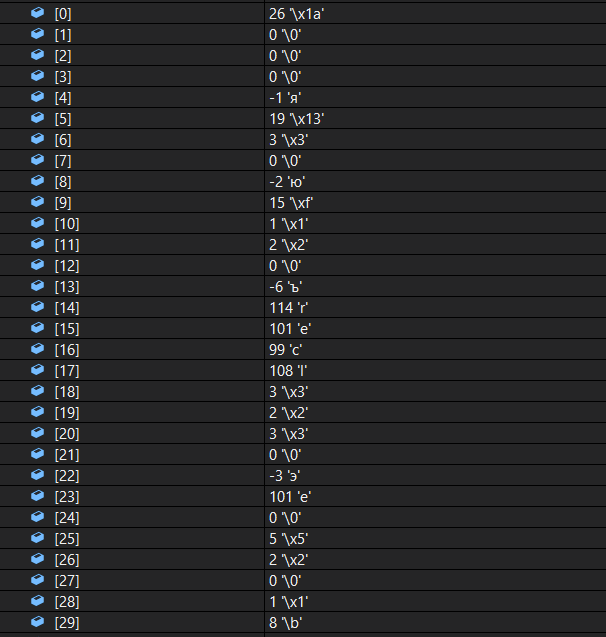
\includegraphics[scale = 0.5]{src/Screenshot_7.png}}}\\

\pagebreak

После преобразования получилась длинная последовательность, во много раз превышающая исходный файл. Это произошло потому, что дерево сохраняется не оптимально и занимает в данном примере 65 байта. Формат хранения дерева: сначала следует символ с вершины файла, после чего следует либо 1, либо 0 в зависимости от направления перехода при обходе дерева:

{\center{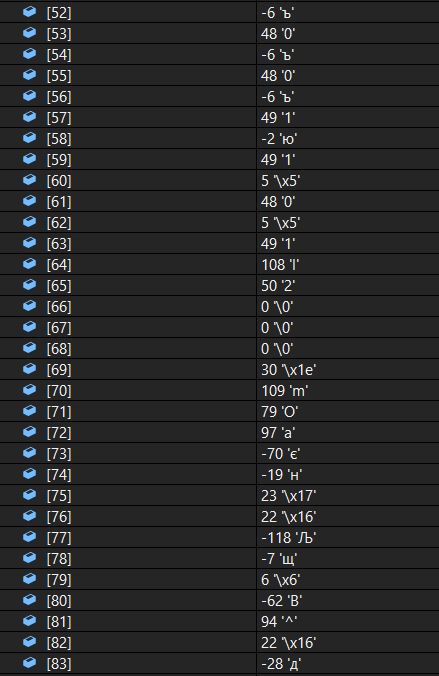
\includegraphics[scale = 0.55]{src/Screenshot_8.png}}}
{\center{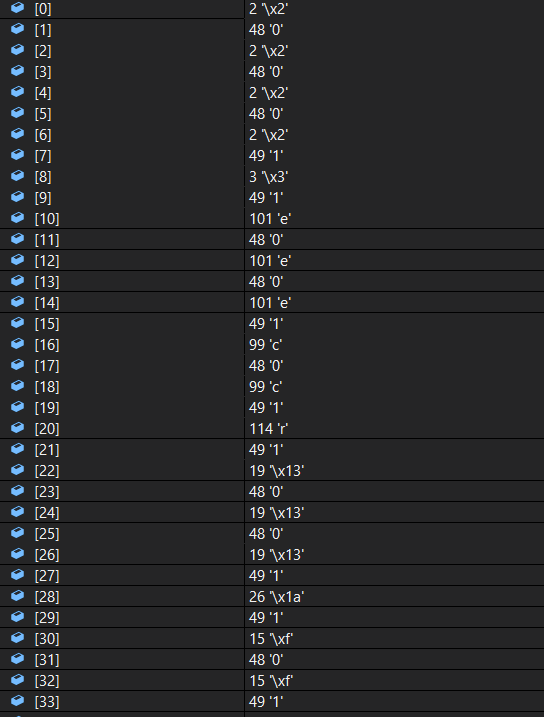
\includegraphics[scale = 0.6]{src/Screenshot_9.png}}}
{\center{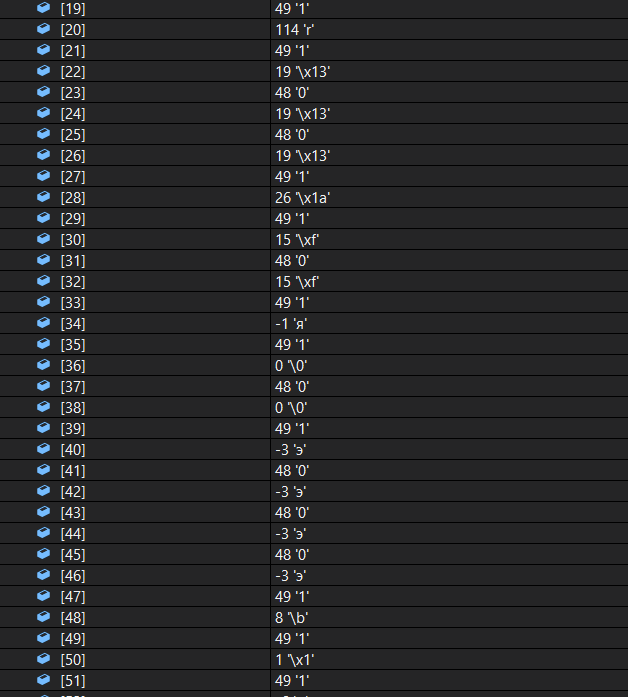
\includegraphics[scale = 0.55]{src/Screenshot_10.png}}}\\

Итоговая последовательность записывается в результирующий файл.

\pagebreak

\section{Исходный код}

Структура программы построена таким обрзом, что каждый класс, инкапсулирующий в себе реализацию алгоритма преобразования наследуется от общего класса {\bfseries Compressor}, переопределяя его метод {\it buffer\_encode} и {\it buffer\_decode}. \\
 
Определение класса {\bfseries Compressor} в {\it Compressor.hpp}:

\begin{lstlisting}[language=C++]
class Compressor{
    public:
        Compressor(); 
        Compressor(istream& inpt, ostream& otpt); 
        Compressor(istream* inpt, ostream* otpt); 
        void set_input(istream& inpt); 
        void set_input(istream* inpt); 
        void set_output(ostream* otpt); 
        void set_output(ostream& otpt); 
        uint64_t get_until_size();
        uint64_t get_after_size();
        void encode(); 
        void decode(); 
        virtual ~Compressor(){}; 
                
    protected:
        virtual void buffer_encode() = 0;
        virtual void buffer_decode() = 0;
        uint64_t until_size = 0;
        uint64_t after_size = 0;
        istream* is;
        ostream* os;
        string in_buffer;
        string out_buffer;
        const uint32_t max_buffer_size = 4194304;
};
\end{lstlisting}

Класс {\bfseries RLE} объялен в {\it RLE.hpp} следующим образом:

\begin{lstlisting}[language=C++]
class RLE : public Compressor{
    public:
        RLE();
        RLE(istream& inpt, ostream& otpt);
        RLE(istream* inpt, ostream* otpt);
    protected:
        void buffer_encode() override;
        void buffer_decode() override;

};
\end{lstlisting}

Класс {\bfseries MTF} из {\it MTF.hpp} содержит в себе список {\it alfabet}, реализующий в себе алгоритм, а так же 2 функции позоляющие получить код для входного символа:

\begin{lstlisting}[language=C++]
class MTF : public Compressor{
    public:
        MTF();
        MTF(istream& inpt, ostream& otpt);
        MTF(istream* inpt, ostream* otpt);
        
    protected:
        void buffer_encode() override;
        void buffer_decode() override;
    private:
        list<uint8_t> alfabet;
        uint8_t move_to_front_encode(uint8_t c);
        uint8_t move_to_front_decode(uint8_t c);
};
\end{lstlisting}

Класс {\bfseries Huffman} из {\it Huffman.hpp} имеет функции для подсчета входений симола в файл, создания дерева, его чтения и записи, а таке несколько вспомогательных функций и структур для работы с деревом.

\begin{lstlisting}[language=C++]
class Huffman : public Compressor{
    public:
        Huffman();
        Huffman(istream& inpt, ostream& otpt);
        Huffman(istream* inpt, ostream* otpt);
    protected:
        void buffer_encode() override;
        void buffer_decode() override;
    private:
        typedef struct Node{
            int32_t left;
            int32_t right;
            uint32_t count;
            char value; // has value only if list, else it rubish
        }node;
    
        // comparator for priority queue
        typedef struct functor{
            bool operator()(const pair<int32_t, uint32_t> lhs, const pair<int32_t, uint32_t> rhs){
                return lhs.second > rhs.second;
            }
        }comparator;

        // TREE (too lazy create new structure):
        int32_t tree = -1; // root
        vector<node> vertex; // vector of vertexes of tree
        // AND OF TREE
        
        void tree_create(); // create tree of encoding
        void tree_from_input(uint32_t& i); // create tree from input for decoding
        void tree_write(int32_t obj); // write tree in output
        void count_table(map<char, uint32_t>& table_of_counts); // count simbols
        void create_encode_table(map<char, vector<uint8_t>>& encode_table);
        void depth_walker(int32_t obj ,vector<uint8_t>& vec, map<char, vector<uint8_t>>& mp);  
};
\end{lstlisting}

Класс {\bfseries BWT} из {\it BWT.hpp} содержит в себе функцию построения суффиксного массива и позицию исхоной строки в таблице сдигов. 

\begin{lstlisting}[language=C++]
class BWT : public Compressor{
    public:
        BWT();
        BWT(istream& inpt, ostream& otpt);
        BWT(istream* inpt, ostream* otpt);
    protected:
        void buffer_encode() override;
        void buffer_decode() override;
    private:
        uint32_t position; // position in sorted cyclic table
        uint32_t count_suff_array(vector<uint32_t>& array); // returns position
};
\end{lstlisting}

\begin{lstlisting}[language=C++]
#include "BWT.hpp"

using namespace std;



BWT::BWT() : Compressor(){}

BWT::BWT(istream& inpt, ostream& otpt) : Compressor(inpt, otpt){}

BWT::BWT(istream* inpt, ostream* otpt) : Compressor(inpt, otpt){}

// O(nlogn) construct from https://e-maxx.ru/algo/suffix_array
// it will array of sorted cyclics - GREAT

uint32_t BWT::count_suff_array(vector<uint32_t>& array){
    uint32_t n = in_buffer.size();
    array.resize(n);

    // equalent classes 
    vector<uint32_t> equality(n);
    uint32_t classes = 0;

    // help vectors
    vector<uint32_t> second_array(n), helper(n);

    // second_array - sorted positions of second parts of new substrings
    // helper - new classes of equality

    // we coding in_buffer fully
    vector<uint32_t> count(256, 0);
    // 0 phase - sort chars in string with count sort
    for(uint32_t i = 0; i < n; ++i){
        ++count[static_cast<uint8_t>(in_buffer[i])];
    }
    for(uint32_t i = 1; i < 256; ++i){
        count[i] += count[i - 1];
    }
    for(uint32_t i = 0; i < n; ++i){
        array[--count[static_cast<uint8_t>(in_buffer[i])]] = i;
    }
    equality[array[0]] = 0;
    
    for(uint32_t i = 1; i < n; ++i){
        if(in_buffer[array[i]] != in_buffer[array[i-1]]){
            ++classes;
        }
        equality[array[i]] = classes;
    }
    ++classes;

    // all another k phases (k = h + 1)

    for(uint32_t h = 0; (1u << h) < n; ++h){
        // second_array - includes old sort positions for string with lenght 2^(k-1)
        // now we should get new sort positions for string with lenght 2^(k)
        // for this we can do radix sort for strings S_k[i] = (S_(k-1)[i], S_(k-1)[i+2^(k-1)])
        // but sort of strings S_k[i] by second positions we can get as second_array[i] = p[i] - 2^(k-1) 
        for(uint32_t i = 0; i < n; ++i){
            second_array[i] = array[i] < (1u << h) ? array[i] + (n - (1 << h)) : array[i] - (1 << h);
        }

        count.assign(classes, 0);

        // and count sort by first positions
        for(uint32_t i = 0; i < n; ++i){
            ++count[equality[second_array[i]]];
        }
        for(uint32_t i = 1; i < classes; ++i){
            count[i] += count[i - 1];
        }
        for(uint32_t i = n - 1; i > 0; --i){
            array[--count[equality[second_array[i]]]] = second_array[i];
        }
        array[--count[equality[second_array[0]]]] = second_array[0];

        helper[array[0]] = 0;
        classes = 0;

        // define classes of equlity
        for(uint32_t i = 1; i < n; ++i){
            // second - second position of new strings
            uint32_t second1 = (array[i] + (1u << h)) >= n ? 
                array[i] + (1u << h) - n : 
                array[i] + (1u << h); 
            uint32_t second2 = array[i - 1] + (1u << h) >= n ? 
                array[i - 1] + (1u << h) - n : 
                array[i - 1] + (1u << h);

            if(equality[array[i]] != equality[array[i - 1]] || equality[second1] != equality[second2]){
                ++classes;
            }
            helper[array[i]] = classes;
        }
        ++classes;
        equality = helper;
    }
    return equality[0];
}

void BWT::buffer_encode(){
    vector<uint32_t> suf_array;
    position = count_suff_array(suf_array);
    for(uint32_t i = 0; i < in_buffer.size(); ++i){
        if(suf_array[i] > 0){
            out_buffer.push_back(in_buffer[suf_array[i] - 1]);
        }else{
            out_buffer.push_back(in_buffer[in_buffer.size() - 1]);
        }
    }

    uint32_t pos = position;
    uint32_t s_mask = 1 << 8; --s_mask; // 00000000000000000000000011111111

    uint8_t byte4 = static_cast<uint8_t>(pos & s_mask);
    pos >>= 8;
    uint8_t byte3 = static_cast<uint8_t>(pos & s_mask);
    pos >>= 8;
    uint8_t byte2 = static_cast<uint8_t>(pos & s_mask);
    pos >>= 8;
    uint8_t byte1 = static_cast<uint8_t>(pos & s_mask);

    out_buffer.push_back(static_cast<char>(byte1));
    out_buffer.push_back(static_cast<char>(byte2));
    out_buffer.push_back(static_cast<char>(byte3));
    out_buffer.push_back(static_cast<char>(byte4));
}

// TO DO:
// change algo for stay in_buffer without changes

void BWT::buffer_decode(){
    // Reading position number from end of file and pop this number for stay in_buffer as string for decode
    position = 0;
    for(uint8_t i = 0; i < sizeof(uint32_t); ++i){
        uint8_t byte = static_cast<uint8_t>(in_buffer[in_buffer.size() - 1 - i]);
        position |= (static_cast<uint32_t>(byte) << (i * 8));
    }

    // DECODE:
    // this algo i get from https://neerc.ifmo.ru/wiki/index.php?title=Преобразование_Барроуза-Уилера
    const uint32_t alphabet = 256;
    const uint32_t n = in_buffer.size() - sizeof(uint32_t);
    vector<uint32_t> count(alphabet, 0);
    vector<uint32_t> t(n);

    // count sort in_buffer and save positions in t

    for(uint32_t i = 0; i < n; ++i){
        ++count[static_cast<uint8_t>(in_buffer[i])];
    }

    uint32_t sum = 0;
    for(uint32_t i = 0; i < alphabet; ++i){
        sum += count[i];
        count[i] = sum - count[i];
    }

    for(uint32_t i = 0; i < n; ++i){
        t[count[static_cast<uint8_t>(in_buffer[i])]++] = i;
    }

    // decode in_buffer using t in out_buffer
    out_buffer.resize(n);
    uint32_t j = t[position];
    for(uint32_t i = 0; i < n; ++i){
        out_buffer[i] = in_buffer[j];
        j = t[j];
    }
}
\end{lstlisting}

\begin{lstlisting}[language=C++]
#include "Huffman.hpp"

using namespace std;


Huffman::Huffman() : Compressor(){}

Huffman::Huffman(istream& inpt, ostream& otpt) : Compressor(inpt, otpt){}

Huffman::Huffman(istream* inpt, ostream* otpt) : Compressor(inpt, otpt){}


void Huffman::buffer_decode(){
    tree = -1;
    vertex.clear();
    uint32_t i = 0;
    // get tree from input
    tree_from_input(i);

    uint32_t size = 0;

    // Reading size of decoded buffer
    for(uint8_t j = 0; j < 4; ++j){
        // read 1 byte
        uint8_t byte = static_cast<uint8_t>(in_buffer[i++]);
        size |= static_cast<uint32_t>(byte) << (8*(3 - j)); // insert bits on needed positions
    }

    // DECODE:
    // counter of simbols needs for stop decode
    uint32_t j = 0; 
    int32_t it = tree;
    for(; i < in_buffer.size(); ++i){
        // reading byte of information:
        uint8_t bits_of_code = in_buffer[i];
        // create mask for reading bits
        uint8_t mask = 1 << 7; // 10000000
        // reading bits
        for(uint8_t k = 0; k < 8 && j < size; ++k){
            // if bit - 1 => go right
            if(bits_of_code & mask){
                it = vertex[it].right;
            }else{
            // if bit - 0 => go left
                it = vertex[it].left;
            }
            // if in list => push decoded simbol in output
            if(vertex[it].left < 0){
                out_buffer.push_back(vertex[it].value);
                // and go back in root
                it = tree;
                // apdate counter of simbols
                ++j;
            }
            // update mask for read next bit
            mask >>= 1;
        }
    }
}


void Huffman::buffer_encode(){
    tree = -1;
    vertex.clear();
    // At first create tree for encode
    tree_create();
    // At second write tree in file
    tree_write(tree);
    // it simbol for end of tree 
    // cant do without this but too lazy
    out_buffer.push_back('2'); // simbol of tree end

    // Create table of simbols codes:
    map<char, vector<uint8_t>> encode_table;
    create_encode_table(encode_table);

    // Save size of buffer:

    uint32_t size = in_buffer.size();

    uint32_t s_mask = 1 << 8; --s_mask;

    uint8_t byte4 = static_cast<uint8_t>(size & s_mask);
    size >>= 8;
    uint8_t byte3 = static_cast<uint8_t>(size & s_mask);
    size >>= 8;
    uint8_t byte2 = static_cast<uint8_t>(size & s_mask);
    size >>= 8;
    uint8_t byte1 = static_cast<uint8_t>(size & s_mask);


    out_buffer.push_back(static_cast<char>(byte1));

    out_buffer.push_back(static_cast<char>(byte2));

    out_buffer.push_back(static_cast<char>(byte3));

    out_buffer.push_back(static_cast<char>(byte4));



    // ENCODING:

    // byte for put in output
    uint8_t bits_of_code = 0;
    uint8_t mask = 1 << 7; // 10000000
    // reaing simbols for encode
    for(uint32_t i = 0; i < in_buffer.size(); ++i){
        // get code of input simbol
        vector<uint8_t>& simbol_code = encode_table[in_buffer[i]];
        // insert code in byte 
        for(uint8_t k = 0; k < simbol_code.size(); ++k){
            // if bit code - 1 => put 1 on needed position(else nothing to do)
            if(simbol_code[k]){
                bits_of_code |= mask;
            }
            // get new position for bit
            mask >>= 1;
            // if mask - 00000000 => put encoded byte in output and go to encode new byte
            if(!mask){
                out_buffer.push_back(static_cast<char>(bits_of_code));

                mask = 1 << 7;
                bits_of_code = 0;
            }
        }
    }
    // if we encoded last simbols but didnt wrote => writing them
    if(mask < (1 << 7)){ 
        out_buffer.push_back(static_cast<char>(bits_of_code));
    }
}


// this function needs for walking in tree and construct code table of simbols  
void Huffman::depth_walker(int32_t obj ,vector<uint8_t>& vec, map<char, vector<uint8_t>>& mp){
    // Wlking in tree and collect way in vector
    // And after that save way for all alfabet simbols 
    if(vertex[obj].left >= 0){
        vec.push_back(0);
        depth_walker(vertex[obj].left, vec, mp);
        vec.pop_back();
        vec.push_back(1);
        depth_walker(vertex[obj].right, vec, mp);
        vec.pop_back();
    }else{
        mp[vertex[obj].value] = vec;
    }
}


void Huffman::create_encode_table(map<char, vector<uint8_t>>& encode_table){
    // DEPTH WALK FOR CREATE ENCODE TABLE
    vector<uint8_t> vec;
    depth_walker(tree, vec, encode_table);
}


void Huffman::tree_write(int32_t obj){
    // Main idea: when we go left put 0
    // when we come to node put value of node
    // when go right put 1 
    // P.S. something like this i made in lab2

    // value
    out_buffer.push_back(vertex[obj].value);

    if(vertex[obj].left >= 0){
        out_buffer.push_back('0');

        tree_write(vertex[obj].left);
    }else{
        // if left - null => right - null in our tree
        return;
    }
    out_buffer.push_back('1');
    tree_write(vertex[obj].right);
}

void Huffman::tree_from_input(uint32_t& i){
    // it very bed code for unerstning but i will try to explain:
    // We construct tree by path simbols: 0 - go left, 1 - go right, 2 - end of building
    // this simbols - instruction to go in depth walking

    // in structure of tree we have not useful for us attribute: count
    // we will save in it index of vertex for up move in depth walking
    // (it not good idea may be, but working)

    // At first create root:
    vertex.push_back(Huffman::node{-1, -1, 0, in_buffer[i++]});
    tree = static_cast<int32_t>(vertex.size() - 1);
    int32_t it = tree;

    // depth walking:
    while(1){
        // if go left: 
        // 1) create new node
        // 2) save in new node index of father in vertex vector
        // 3) init left and go
        if(in_buffer[i] == '0'){
            ++i;
            vertex.push_back(Huffman::node{-1, -1, static_cast<uint32_t>(it), in_buffer[i++]});
            // create left
            vertex[it].left = static_cast<int32_t>(vertex.size() - 1);
            // go left
            it = vertex[it].left;
            continue;
        }
        // if go right:
        // 1) move up to vertex for create right child for go right 
        // 2) create new Huffman::node
        // 3) set here upper travel as upper travel for her father
        // 4) init right and go 
        if(in_buffer[i] == '1'){
            ++i;
            // move up
            it = vertex[it].count;
            // here set father travel
            vertex.push_back(Huffman::node{-1, -1, vertex[it].count, in_buffer[i++]});
            // create node 
            vertex[it].right = vertex.size() - 1;
            // go right
            it = vertex[it].right;
        }
        // if read 2 => end of walking
        if(in_buffer[i] == '2'){
            ++i;
            return;
        }
    }
}

void Huffman::tree_create(){
    // table of counts simbol repeats in buffer
    map<char, uint32_t> table_of_counts;
    count_table(table_of_counts);

    // priority queue for Huffman algo(may be not too fast as custom, but create custom lazy)
    //priority_queue<Huffman::node, vector<Huffman::node>, comparator> que;
    priority_queue<pair<int32_t, uint32_t>, vector<pair<int32_t, uint32_t>>, comparator> que;

    // create and insert basic nodes(lists) in queue
    for(auto it : table_of_counts){
        vertex.push_back(Huffman::node{-1, -1, it.second, it.first});
        que.push(pair<int32_t, uint32_t>(vertex.size()-1, vertex.back().count));
    }

    // situation when only 1 simbol in alfabet: will encode all simbols as 0
    // it exception from rule:)
    if(que.size() == 1){
        vertex.push_back(Huffman::node{-1, -1, vertex[0].count, static_cast<char>(vertex[0].value+1)});
        vertex.push_back(Huffman::node{0, 1, vertex[0].count, vertex[0].value});
        tree = 2;
        return;
    }

    // build tree from queue: itteration while not 1 elem in queue
    while(que.size() > 1){
        // take 2 nodes with less counts
        int32_t left = que.top().first; que.pop();
        int32_t right = que.top().first; que.pop();
        // create new node with left and right childs
        vertex.push_back(Huffman::node{left, right, vertex[left].count + vertex[right].count, vertex[left].value});
        // push new node to queue
        que.push(pair<int32_t, uint32_t>(vertex.size()-1, vertex.back().count));
    }
    
    tree = que.top().first;
    que.pop(); // clear queue(not need)
}


// count table of repeats in buffer
void Huffman::count_table(map<char, uint32_t>& table_of_counts){
    for(uint32_t i = 0; i < in_buffer.size(); ++i){
        ++table_of_counts[in_buffer[i]];
    }
}
\end{lstlisting}

\begin{lstlisting}[language=C++]
#include "MTF.hpp"

using namespace std;

// TO DO

// change algo for do possible count and insert numbers more than 127

MTF::MTF() : Compressor(){}

MTF::MTF(istream& inpt, ostream& otpt) : Compressor(inpt, otpt){}

MTF::MTF(istream* inpt, ostream* otpt) : Compressor(inpt, otpt){}

void MTF::buffer_encode(){
    alfabet.clear();
    // init alfabet
    for(uint16_t i = 0; i < 256; ++i){
        alfabet.push_back(static_cast<uint8_t>(i));
    }

    // ENCODE:
    for(char c : in_buffer){
        out_buffer.push_back(
            static_cast<char>(
                move_to_front_encode(
                    static_cast<uint8_t>(c)
                )
            )
        );
    }
}

void MTF::buffer_decode(){
    alfabet.clear();
    // init alfabet:
    for(uint16_t i = 0; i < 256; ++i){
        alfabet.push_back(static_cast<uint8_t>(i));
    }

    // DECODE:
    for(char c : in_buffer){
        out_buffer.push_back(
            static_cast<char>(
                move_to_front_decode(
                    static_cast<uint8_t>(c)
                )
            )
        );
    }
}

uint8_t MTF::move_to_front_encode(uint8_t c){
    uint8_t i = 0;
    for (auto it = alfabet.begin(); ; ++it, ++i){
        if(*it == c){
            alfabet.erase(it);
            break;
        }
    }
    alfabet.push_front(c);
    return i;
}


uint8_t MTF::move_to_front_decode(uint8_t c){
    auto it = alfabet.begin();
    advance(it, c);
    uint8_t i = *it;
    alfabet.erase(it);
    alfabet.push_front(i);
    return i;
}
\end{lstlisting}

\begin{lstlisting}[language=C++]
#include "RLE.hpp"

using namespace std;

// TO DO

// change algo for do possible count and insert numbers more than 127

RLE::RLE() : Compressor(){}

RLE::RLE(istream& inpt, ostream& otpt) : Compressor(inpt, otpt){}

RLE::RLE(istream* inpt, ostream* otpt) : Compressor(inpt, otpt){}

void RLE::buffer_encode(){
    int8_t count = 0;
    string buffer;
    buffer.clear();
    char last_ch = in_buffer[0]; // set unique
    // Always save last char from in buffer
    for(uint32_t i = 1; i < in_buffer.size(); ++i){
        // if repeat
        if(in_buffer[i] == last_ch){
            // if its first repeat, push in output unique char until repeat chars
            if(count < 0){
                out_buffer.push_back(static_cast<char>(count));
                out_buffer += buffer;
                buffer.clear();
                count = 0;
            }
            // we have +1 repeating char - last char
            ++count;
            // if num of repeats until this char = 127 => push back this info and go next
            if(count == INT8_MAX){
                out_buffer.push_back(static_cast<char>(count));
                out_buffer.push_back(last_ch);
                count = 0;
            }
        }else{ // - if not repeat
            // if its first unique char => push count and char of repeats
            if(count > 0){
                // count + 1 because last char also repeated
                ++count;
                out_buffer.push_back(static_cast<char>(count));
                out_buffer.push_back(last_ch);
                count = 0;
            }else{
                // if its not first unique char - push_back it in temp buffer
                // and increment count of unique
                --count;
                buffer.push_back(last_ch);
                if (count == INT8_MIN){
                    out_buffer.push_back(static_cast<char>(count));
                    out_buffer += buffer;
                    buffer.clear();
                    count = 0;
                }
            }
            
        }
        last_ch = in_buffer[i];
    }
    // we should define group for last char of input and 
    // push nesassary info in output
    if(count < 0){
        --count;
        buffer.push_back(last_ch);
        out_buffer.push_back(static_cast<char>(count));
        out_buffer += buffer;
    }else{
        ++count;
        out_buffer.push_back(static_cast<char>(count));
        out_buffer.push_back(last_ch);
    }
    
}

void RLE::buffer_decode(){
    uint32_t i = 0;
    int8_t count = 0;
    while(i < in_buffer.size()){
        count = static_cast<int8_t>(in_buffer[i++]);
        while(count < 0){
            out_buffer.push_back(in_buffer[i++]);
            ++count;
        }
        if(count > 0){
            char tmp = in_buffer[i++];
            while (count > 0){
                out_buffer.push_back(tmp);
                --count;
            }
        }
    }
}
\end{lstlisting}

\begin{lstlisting}[language=C++]
#include "Arhivator.hpp"
#include <cstdio>

using namespace std;

Arhivator::Arhivator(){
    stdinput = true;
    decode = false;
    stdoutput = false;
    hard = false;
    easy = false;
    keep = false;
    recursive = false;
    check = false;
    information = false;
    path.clear();
}

void Arhivator::set_stdoutput(){
    stdoutput = true;
}

void Arhivator::set_path(string& str){
    path = str;
    if(str.empty()){
        stdinput = true;
    }else{
        stdinput = false;
    }
}

void Arhivator::set_hard(){
    hard = true;
    if(easy){
        hard = false;
    }
}

void Arhivator::set_easy(){
    easy = true;
    if(hard){
        hard = false;
    }
}

void Arhivator::set_recursive(){
    recursive = true;
}

void Arhivator::set_information(){
    information = true;
}

void Arhivator::set_check(){
    check = true;
}

void Arhivator::set_keep(){
    keep = true;
}

void Arhivator::set_decode(){
    decode = true;
}

void Arhivator::start(){
    if(stdinput){
        stdoutput = true;
    }
    if(information){
        if(stdinput){
            check_info(cin);
        }else{
            ifstream is(path, ios::in | ios::binary);
            if(!is){
                throw MyException(path + " not a file");
            }
            check_info(is);
            is.close();
        }
        return;
    }
    if(check){
        if(stdinput){
            check_zip(cin);
        }else{
            ifstream is(path, ios::in | ios::binary);
            if(!is){
                throw MyException(path + " not a file");
            }
            if(check_zip(is)){
                cout << "True" << endl;
            }else{
                cout << "False" << endl;
            }
            is.close();
        }
        return;
    }
    if(recursive){
        throw MyException("Not Ready Yet");
    }
    if(hard || easy){
        throw MyException("Not Ready Yet");
    }
    if(decode){
        decode_file(path);
        return;
    }else{
        encode_file(path);
        return;
    }
}

void Arhivator::encode_file(string& path){
    ifstream inpt(path, ios::in | ios::binary);
    if(!inpt){
        throw MyException(path + " is not a file");
    }
    if(!stdoutput){
        ofstream otpt(path + ".gz", ios::out | ios::binary);
        encode_stream(inpt, otpt);
        otpt.close();
        if(!keep){
            remove(path.c_str());
        }
    }else{
        encode_stream(inpt, cout);
        if(!keep){
            remove(path.c_str());
        }
    }
}

void Arhivator::decode_file(string& path){
    string suf = path.substr(path.size() - 3, 3);
    if(suf != ".gz"){
        throw MyException(path + " has unknown suffix");
    }
    ifstream inpt(path, ios::in | ios::binary);
    if(!inpt){
        throw MyException(path + " is not a file");
    }
    
    if(!stdoutput){
        ofstream otpt(path.substr(0, path.size() - 3), ios::out | ios::binary | ios::trunc);
        decode_stream(inpt, otpt);
        otpt.close();
        if(!keep){
            remove(path.c_str());
        }
    }else{
        decode_stream(inpt, cout);
        if(!keep){
            remove(path.c_str());
        }
    }
}

void Arhivator::check_info(istream& is){
    string pre;
    pre.resize(prefix.size());
    uint64_t old_size, new_size;
    is.read(&pre[0], prefix.size());
    if(prefix != pre){
        throw MyException("not in zip format");
    }
    is.read(reinterpret_cast<char *>(&old_size), sizeof(uint64_t));
    is.read(reinterpret_cast<char *>(&new_size), sizeof(uint64_t));
    if(!is || !check_hash(is)){
        throw MyException("not in zip format");
    }
    cout << "Unompressed size: " << old_size << endl;
    cout << "Compressed size: " << new_size << endl;
    cout << "Ratio: " 
    << 100.0 * static_cast<double>(old_size - new_size) 
    / static_cast<double>(old_size) << "%" << endl; 
}

// will coding streams: 
// is - stream of input file(or stdin), os -steam of output file(or stdout)
void Arhivator::encode_stream(istream& is, ostream& os){
    Compressor* cmp;
    string tmpnm = path;
    string file1 = tmpnm + ".1";
    string file2 = tmpnm + ".2";
    string file3 = tmpnm + ".3";
    string file4 = tmpnm + ".4";
    ifstream tmp_in;
    ofstream tmp_out;
    uint64_t input_size = 0;
    uint64_t output_size = 0;
    uint32_t hash_c = 0;

    // ENCODING:

    // 1 step
    tmp_out.open(file1, ios::out | ios::binary);
    cmp = new BWT(is, tmp_out);
    cmp->encode();
    input_size = cmp->get_until_size();
    delete cmp;
    tmp_out.close(); // TODO exceptions

    // 2 step
    tmp_in.open(file1, ios::in | ios::binary);
    tmp_out.open(file2, ios::out | ios::binary);
    cmp = new MTF(tmp_in, tmp_out);
    cmp->encode();
    delete cmp;
    tmp_in.close();
    tmp_out.close();
    remove(file1.c_str());

    // 3 step
    tmp_in.open(file2, ios::in | ios::binary);
    tmp_out.open(file3, ios::out | ios::binary);
    cmp = new RLE(tmp_in, tmp_out);
    cmp->encode();
    delete cmp;
    tmp_in.close();
    tmp_out.close();
    remove(file2.c_str());

    // 4 step
    tmp_in.open(file3, ios::in | ios::binary);
    tmp_out.open(file4, ios::out | ios::binary);
    cmp = new Huffman(tmp_in, tmp_out);
    cmp->encode();
    // size of encoded input
    output_size = cmp->get_after_size();
    delete cmp;
    tmp_in.close();
    tmp_out.close();
    remove(file3.c_str());

    // gen and add info into output
    // 1 - add constant prefix for check gzip format
    os.write(prefix.c_str(), prefix.size());
    // 2 - add old size of file
    os.write(reinterpret_cast<const char*>(&input_size), sizeof(uint64_t));
    // 3 - count new size of file
    // encoded inpt + preix size + 2 sizes + hash of file
    output_size += 2 * sizeof(uint64_t) + prefix.size() + sizeof(uint32_t);
    os.write(reinterpret_cast<const char*>(&output_size), sizeof(uint64_t));
    // 4 - add hash
    tmp_in.open(file4, ios::in | ios::binary);
    hash_c = hash_count(tmp_in);
    // return to start pos
    tmp_in.close();

    os.write(reinterpret_cast<const char*>(&hash_c), sizeof(uint32_t));

    // 5 - insert encoed data at least of file
    tmp_in.open(file4, ios::in | ios::binary);
    from_stream_to_stream(tmp_in, os);
    // and remove old file
    tmp_in.close();
    remove(file4.c_str());
}

void Arhivator::decode_stream(istream& is, ostream& os){
    Compressor* cmp;
    string tmpnm = path;
    string file0 = tmpnm + ".0";
    string file1 = tmpnm + ".1";
    string file2 = tmpnm + ".2";
    string file3 = tmpnm + ".3";
    ifstream tmp_in;
    ofstream tmp_out;

    // CHECK ZIP FORMAT OF FILE

    // Writing all stream in tmp file
    tmp_out.open(file0, ios::out | ios::binary);
    from_stream_to_stream(is, tmp_out);
    tmp_out.close();

    // Check zip format and take pointer to start of encoded data 
    // after special simbols and numbers
    tmp_in.open(file0, ios::in | ios::binary);

    if(!check_zip(tmp_in)){
        throw MyException("not a zip formt");
    }

    tmp_in.close();


    tmp_in.open(file0, ios::in | ios::binary);

    tmp_in.seekg(2*sizeof(uint64_t) + prefix.size() + sizeof(uint32_t), ios::beg);


    // DECODING:
    
    // Decode all characters after specil simbols

    // 1 step
    tmp_out.open(file1, ios::out | ios::binary);
    cmp = new Huffman(tmp_in, tmp_out);
    cmp->decode();
    delete cmp;
    tmp_out.close(); // TODO exceptions
    tmp_in.close();
    remove(file0.c_str());

    // 2 step
    tmp_in.open(file1, ios::in | ios::binary);
    tmp_out.open(file2, ios::out | ios::binary);
    cmp = new RLE(tmp_in, tmp_out);
    cmp->decode();
    delete cmp;
    tmp_in.close();
    tmp_out.close();
    remove(file1.c_str());

    // 3 step
    tmp_in.open(file2, ios::in | ios::binary);
    tmp_out.open(file3, ios::out | ios::binary);
    cmp = new MTF(tmp_in, tmp_out);
    cmp->decode();
    delete cmp;
    tmp_in.close();
    tmp_out.close();
    remove(file2.c_str());

    // 4 step decoding in output
    tmp_in.open(file3, ios::in | ios::binary);
    cmp = new BWT(tmp_in, os);
    cmp->decode();
    delete cmp;
    tmp_in.close();
    remove(file3.c_str());
}

bool Arhivator::check_hash(istream& is){
    uint32_t hash_f = 0;
    if(is){
        is.read(reinterpret_cast<char*>(&hash_f), sizeof(uint32_t));
    }
    uint32_t hash_c = hash_count(is);
    return hash_f == hash_c;
}

bool Arhivator::check_zip(istream& is){
    string buffer;
    buffer.resize(prefix.size());
    if(is){
        is.read(&buffer[0], prefix.size());
        if(buffer != prefix){
            return false;
        }
    }
    uint64_t placebo;
    if(is){
        is.read(reinterpret_cast<char*>(&placebo), sizeof(uint64_t));
    }
    if(is){
        is.read(reinterpret_cast<char*>(&placebo), sizeof(uint64_t));
    }
    return check_hash(is);
}

uint32_t Arhivator::hash_count(istream& is){
    string buffer;
    uint32_t ans = 0;
    buffer.resize(max_size_buffer);
    std::hash<string> func;
    while(is){
        is.read(&buffer[0], max_size_buffer);
        ans += func(buffer);
    }
    return ans;
}

void Arhivator::from_stream_to_stream(istream& is, ostream& os){
    string bufer;
    bufer.resize(max_size_buffer);
    while(is){
        is.read(&bufer[0], max_size_buffer);
        os.write(bufer.c_str(), is.gcount());
    }
}


\end{lstlisting}

\begin{lstlisting}[language=C++]
class BWT : public Compressor{
    public:
        BWT();
        BWT(istream& inpt, ostream& otpt);
        BWT(istream* inpt, ostream* otpt);
    protected:
        void buffer_encode() override;
        void buffer_decode() override;
    private:
        uint32_t position; // position in sorted cyclic table
        uint32_t count_suff_array(vector<uint32_t>& array); // returns position
};
\end{lstlisting}

\begin{lstlisting}[language=C++]
// Made by Max Bronnikov
#ifndef ARHIVATOR_H
#define ARHIVATOR_H

#include <iostream>
#include <fstream>
#include <exception> // для std::exception
#include "Compressors/Compressor.hpp"
#include "Compressors/RLE/RLE.hpp"
#include "Compressors/MTF/MTF.hpp"
#include "Compressors/Huffman/Huffman.hpp"
#include "Compressors/BWT/BWT.hpp"

using namespace std;



class MyException: public std::exception
{
private:
	string m_error;
 
public:
	MyException(string error) : m_error(error){}
 
	const char* what() const noexcept { return m_error.c_str(); } 
};



class Arhivator{
    public:
        Arhivator();
        void set_decode();
        void set_stdoutput();
        void set_path(string& str);
        void set_hard();
        void set_easy();
        void set_keep();
        void set_recursive();
        void set_check();
        void set_information();
        void start();

    private:
        void decode_file(string& path);
        void encode_file(string& path);
        void check_info(istream& is);
        // void decode_dir(const string& path);
        // void encode_dir(const string& path);
        void encode_stream(istream& is, ostream& os);
        void decode_stream(istream& is, ostream& os);
        void from_stream_to_stream(istream& is, ostream& os);
        uint32_t hash_count(istream& is);
        bool check_hash(istream& is);
        bool check_zip(istream& is);

        bool stdinput; // without filename

        bool stdoutput; // -c
        bool hard; // -9
        bool easy; // -1
        bool keep; // -k
        bool recursive; // -r
        bool decode; // -d
        bool check; // -t
        bool information; // -l

        uint32_t max_size_buffer = 4194304; // size of bufer for excange and hash counting
        string path; // file or directory path
        const string prefix = "\3\2\1\0"; // for check format

};

#endif
\end{lstlisting}

\begin{lstlisting}[language=C++]
// Made By Max Bronnikov
#include <iostream>
#include <vector>
#include <string>
#include "Arhivator/Arhivator.hpp"

using namespace std;

// Demo of using Arhivator class

// This Demo light version of gzip
int main(int argc, char const *argv[])
{
    if(argc < 2){
        cout << "gzip: compressed data not written to a terminal." << endl;
        cout << "For help, type: gzip -h" << endl;
        return 0;
    }
    vector<string> vector_of_path;
    Arhivator arhive;

    for(int i = 1; i < argc; ++i){
        if(argv[i][0] == '-'){
            switch (argv[i][1]){
                case 'd':
                    arhive.set_decode();
                    break;
                case '1':
                    arhive.set_easy();
                    break;
                case '9':
                    arhive.set_hard();
                    break;
                case 'l':
                    arhive.set_information();
                    break;
                case 't':
                    arhive.set_check();
                    break;
                case 'r':
                    arhive.set_recursive();
                    break;
                case 'k':
                    arhive.set_keep();
                    break;
                case 'c':
                    arhive.set_stdoutput();
                    break;
                case '\0': 
                    vector_of_path.push_back(string());
                    break;   
                default:
                    break;
            }
        }else{
            vector_of_path.push_back(argv[i]);
        }
    }
    if(vector_of_path.empty()){
        vector_of_path.push_back(string());
    }

    try{
        for(unsigned i = 0; i < vector_of_path.size(); ++i){
            arhive.set_path(vector_of_path[i]);
            arhive.start();
        }
    }catch(std::exception &exeption){
        cerr << "gzip: " << exeption.what() << endl;
        return 0; 
    }

    return 0;
}

\end{lstlisting}

Полный код на моем {\it GitHub: https://github.com/Bronnikoff/DA/tree/master/KP}

\pagebreak

\section{Консоль}
\begin{alltt}
(base) max@max-X550CC:~/DA/KP$ ls
Arhivator  Makefile    SampleSubmission.csv  Train.csv
main.cpp   report.pdf  Test.csv
(base) max@max-X550CC:~/DA/KP$ gzip -k Test.csv Train.csv SampleSubmission.csv 
(base) max@max-X550CC:~/DA/KP$ gzip -l Test.csv.gz Train.csv.gz SampleSubmission.csv.gz 
         compressed        uncompressed  ratio uncompressed_name
            1070430             6991963  84.7% Test.csv
            1403853             7686426  81.7% Train.csv
             251796             1800009  86.0% SampleSubmission.csv
            2726079            16478398  83.5% (totals)
(base) max@max-X550CC:~/DA/KP$ make
g++ -std=c++17 -Wall -pedantic -c Arhivator/Compressors/Compressor.cpp
g++ -std=c++17 -Wall -pedantic -c Arhivator/Arhivator.cpp
g++ -std=c++17 -Wall -pedantic -c Arhivator/Compressors/RLE/RLE.cpp
g++ -std=c++17 -Wall -pedantic -c Arhivator/Compressors/BWT/BWT.cpp
g++ -std=c++17 -Wall -pedantic -c Arhivator/Compressors/Huffman/Huffman.cpp
g++ -std=c++17 -Wall -pedantic -c Arhivator/Compressors/MTF/MTF.cpp
g++ -std=c++17 -Wall -pedantic -c main.cpp
g++ Compressor.o Arhivator.o RLE.o BWT.o Huffman.o MTF.o main.o -o KP
rm -rf *.o
(base) max@max-X550CC:~/DA/KP$ rm *.gz
(base) max@max-X550CC:~/DA/KP$ ./KP Test.csv 
(base) max@max-X550CC:~/DA/KP$ ./KP -l Test.csv.gz 
Unompressed size: 6991963
Compressed size: 1031026
Ratio: 85.2541%
(base) max@max-X550CC:~/DA/KP$ ./KP Train.csv  
(base) max@max-X550CC:~/DA/KP$ ./KP -l Train.csv.gz  
Unompressed size: 7686426
Compressed size: 1285648
Ratio: 83.2738%
(base) max@max-X550CC:~/DA/KP$ ./KP SampleSubmission.csv  
(base) max@max-X550CC:~/DA/KP$ ./KP -l SampleSubmission.csv.gz  
Unompressed size: 1800009
Compressed size: 55916
Ratio: 96.8936%
(base) max@max-X550CC:~/DA/KP$ ./KP test.djvu 
(base) max@max-X550CC:~/DA/KP$ ./KP -l test.djvu.gz 
Unompressed size: 9511403
Compressed size: 9594466
Ratio: 0.0%
(base) max@max-X550CC:~/DA/KP$ ./KP -k report.pdf 
(base) max@max-X550CC:~/DA/KP$ ./KP -l report.pdf.gz 
Unompressed size: 325528
Compressed size: 324174
Ratio: 0.41594%
(base) max@max-X550CC:~/DA/KP$ ./KP -d test.djvu.gz 
(base) max@max-X550CC:~/DA/KP$ gzip -k test.djvu report.pdf 
(base) max@max-X550CC:~/DA/KP$ gzip -l test.djvu.gz report.pdf.gz 
         compressed        uncompressed  ratio uncompressed_name
            9512138             9511403  -0.0% test.djvu
             320366              325528   1.6% report.pdf
            9832504             9836931   0.0% (totals)
(base) max@max-X550CC:~/DA/KP$ gzip -k test1.pdf 
(base) max@max-X550CC:~/DA/KP$ gzip -l test1.pdf.gz 
         compressed        uncompressed  ratio uncompressed_name
             568111              727670  21.9% test1.pdf
(base) max@max-X550CC:~/DA/KP$ ./KP -k test1.pdf 
(base) max@max-X550CC:~/DA/KP$ ./KP -l test1.pdf.gz 
Unompressed size: 727670
Compressed size: 602360
Ratio: 17.2207%
(base) max@max-X550CC:~/DA/KP$ ./KP -k 191110.en.pdf 
(base) max@max-X550CC:~/DA/KP$ ./KP -l 191110.en.pdf.gz 
Unompressed size: 284569
Compressed size: 281107
Ratio: 1.21658%
(base) max@max-X550CC:~/DA/KP$ gzip 191110.en.pdf 
gzip: 191110.en.pdf.gz already exists; do you wish to overwrite (y or n)? y
(base) max@max-X550CC:~/DA/KP$ gzip -l 191110.en.pdf.gz 
         compressed        uncompressed  ratio uncompressed_name
             275139              284569   3.3% 191110.en.pdf
\end{alltt} \\

{\bfserises Рассмотрим полученные результаты} \\

На хорошо сжимаемых данных размер сжатого файла, а значит и эффективность сжатия у моей программы выше чем у $gzip$: \\

{\center{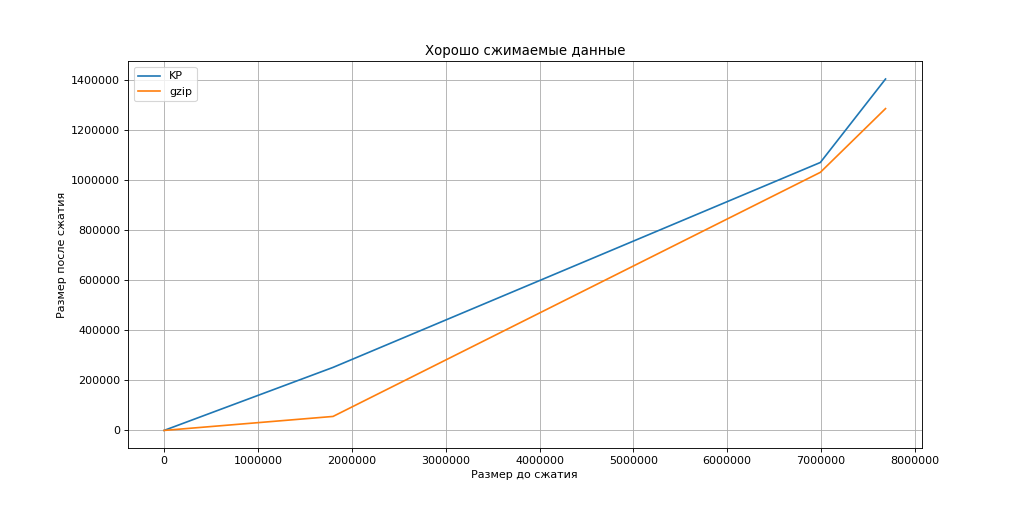
\includegraphics[scale = 0.55]{src/good.png}}} \\

На плохо сжимаемых данных размер сжатого файла, а значит и эффективность сжатия у моей программы ние чем у $gzip$, однако разница незначительна: \\

{\center{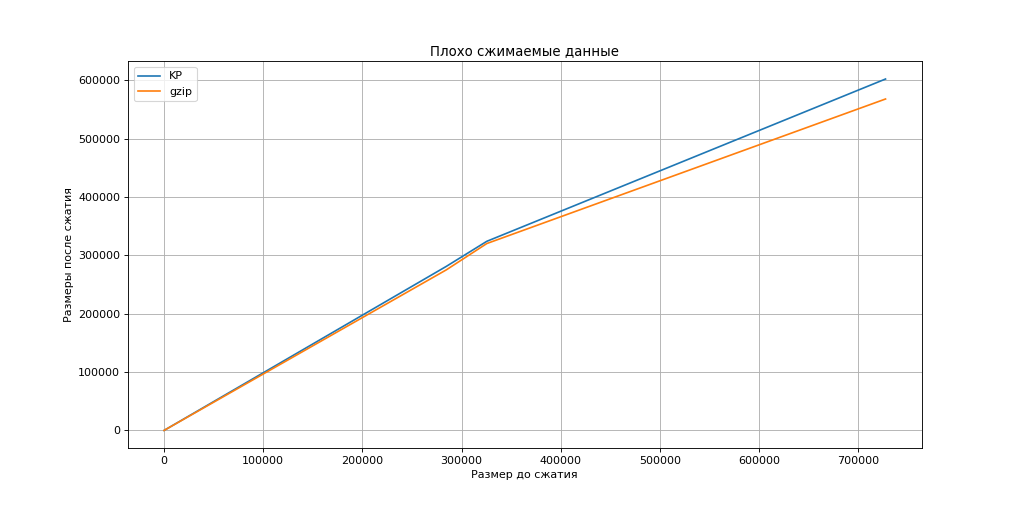
\includegraphics[scale = 0.55]{src/bad.png}}} \\

\pagebreak

